\chapter{SPT-DSFG SEDs}

\begin{figure}
	\centering
	\caption[SEDs of SPT sample (Optically thin)]{SEDs of the SPT sample (optically thin model) and the residuals on the best fitting model. The shaded regions represent the $16$th to $84$th percentiles in the range of SEDs explored during fitting.}
	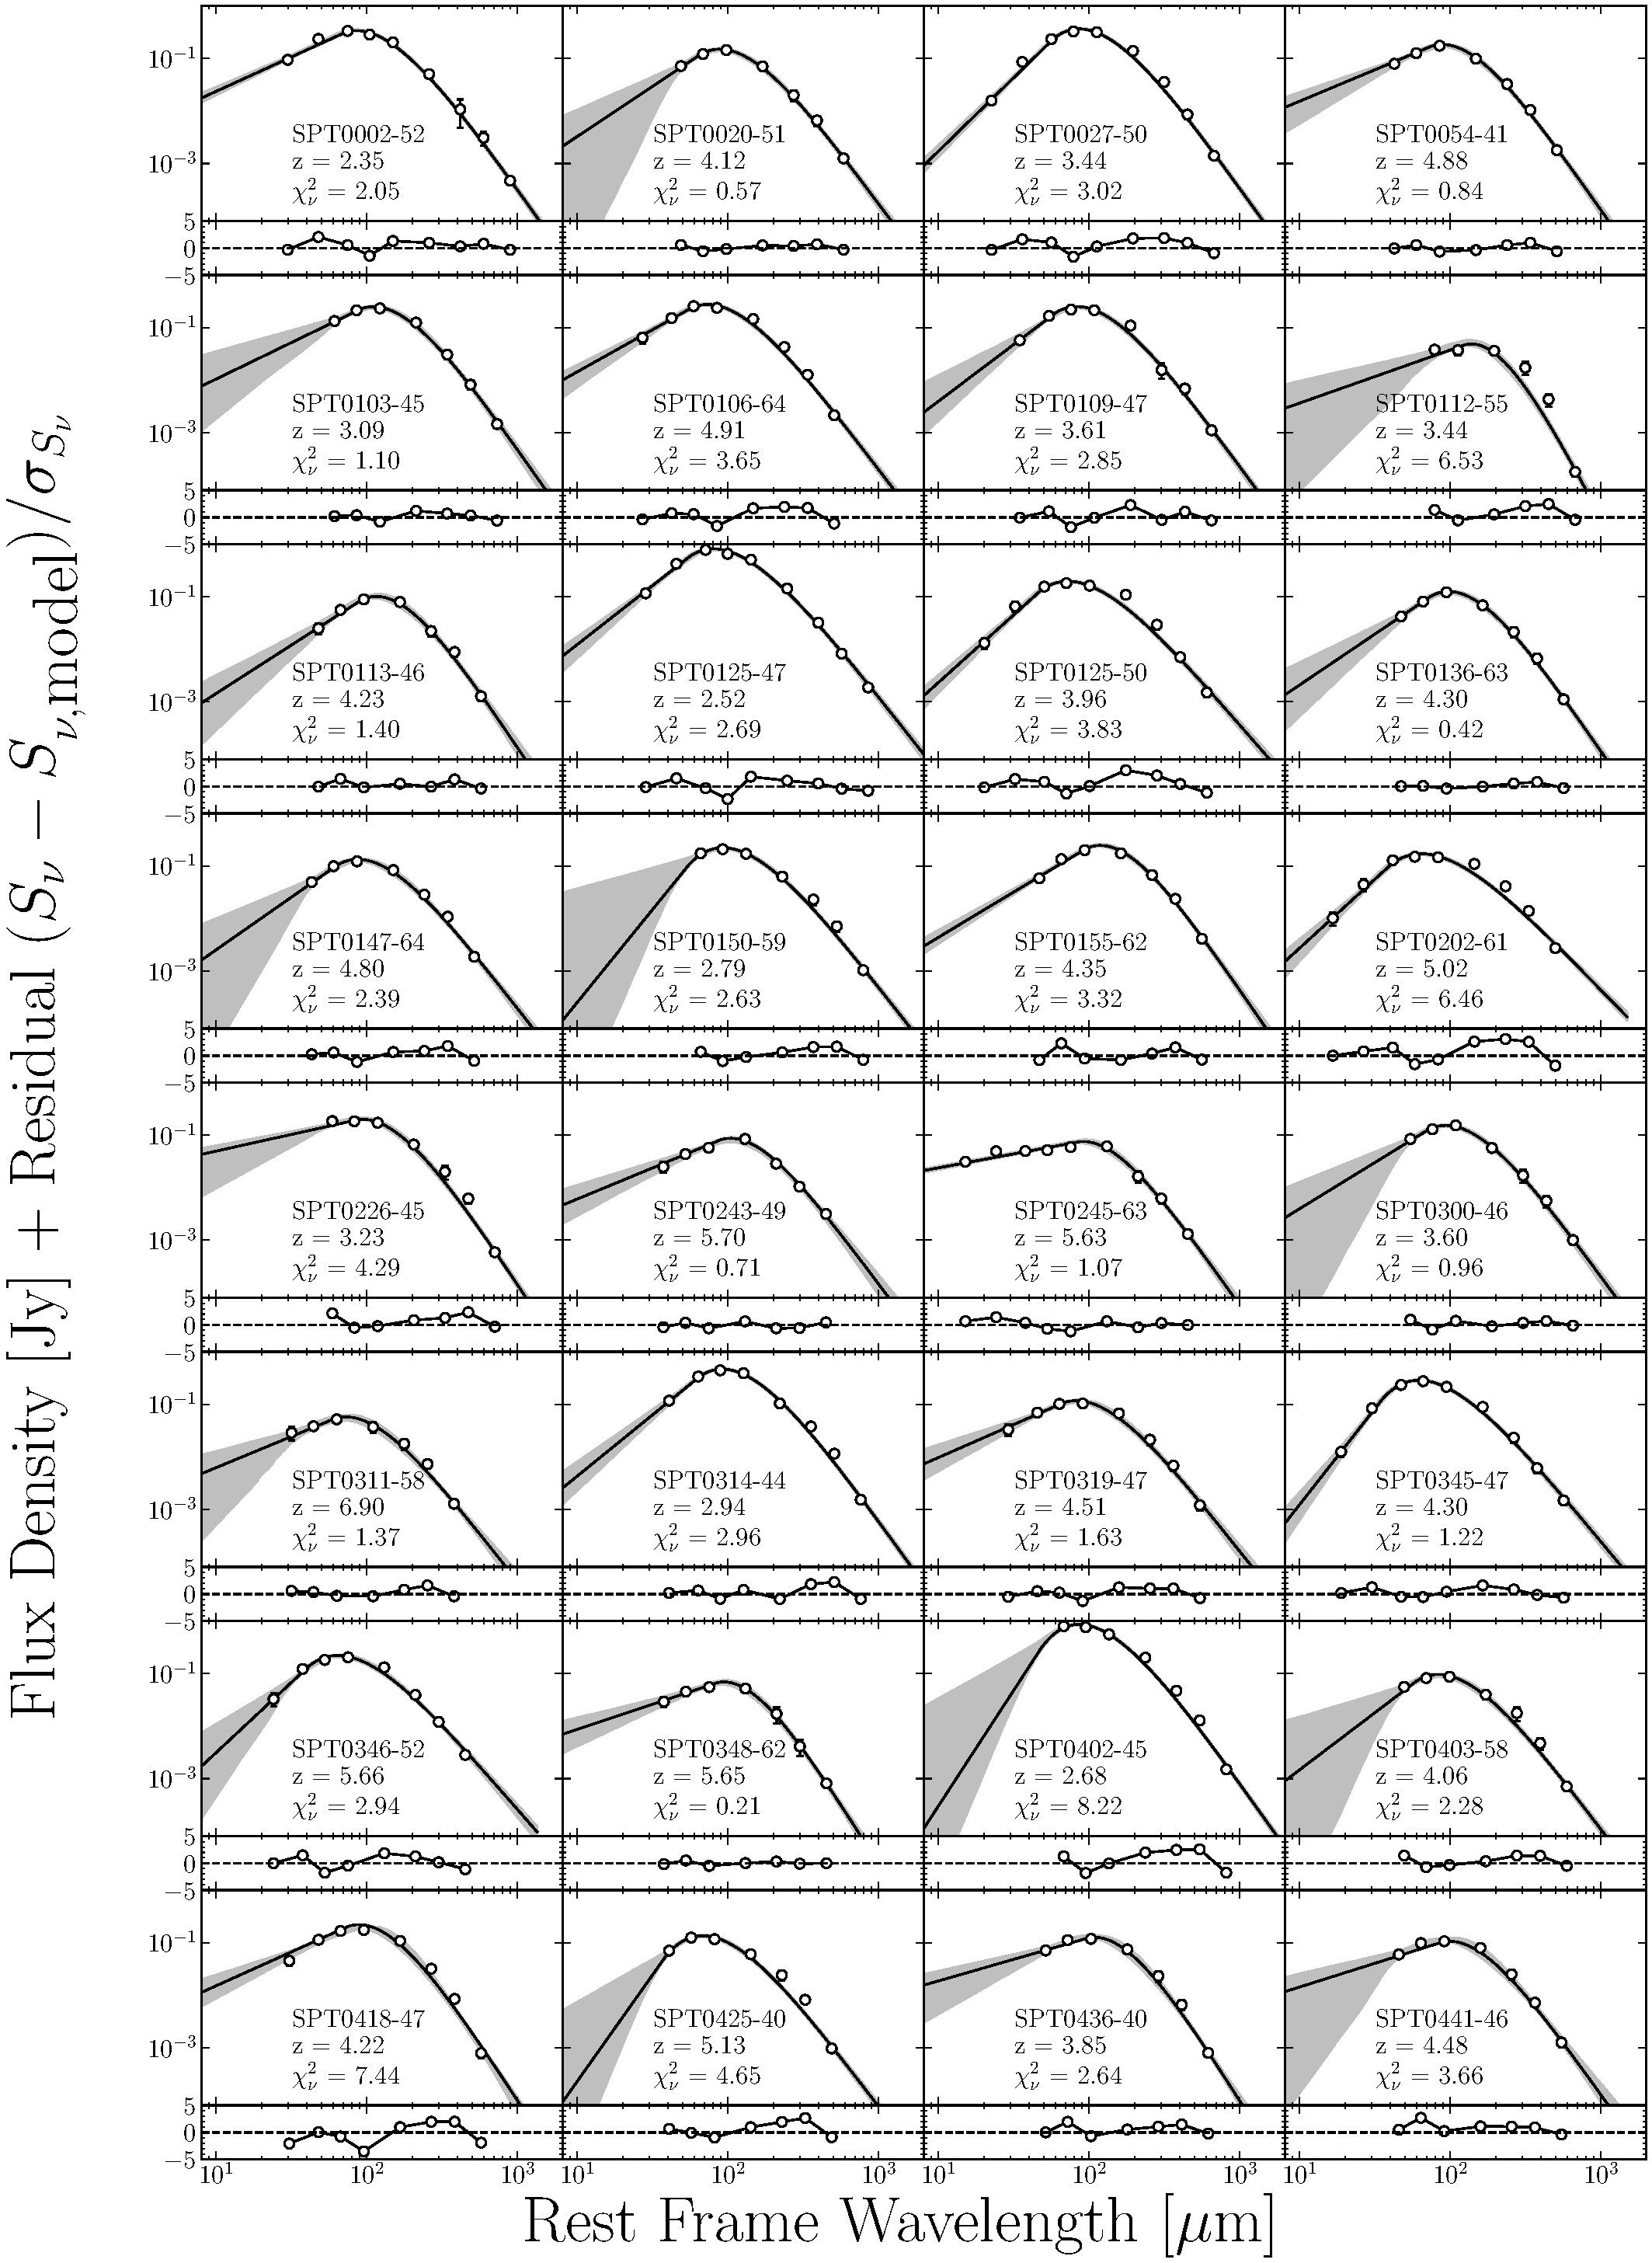
\includegraphics[width=\columnwidth]{Figures/Figure_D_1_part1.pdf}
\end{figure}
\begin{figure}
	\centering
	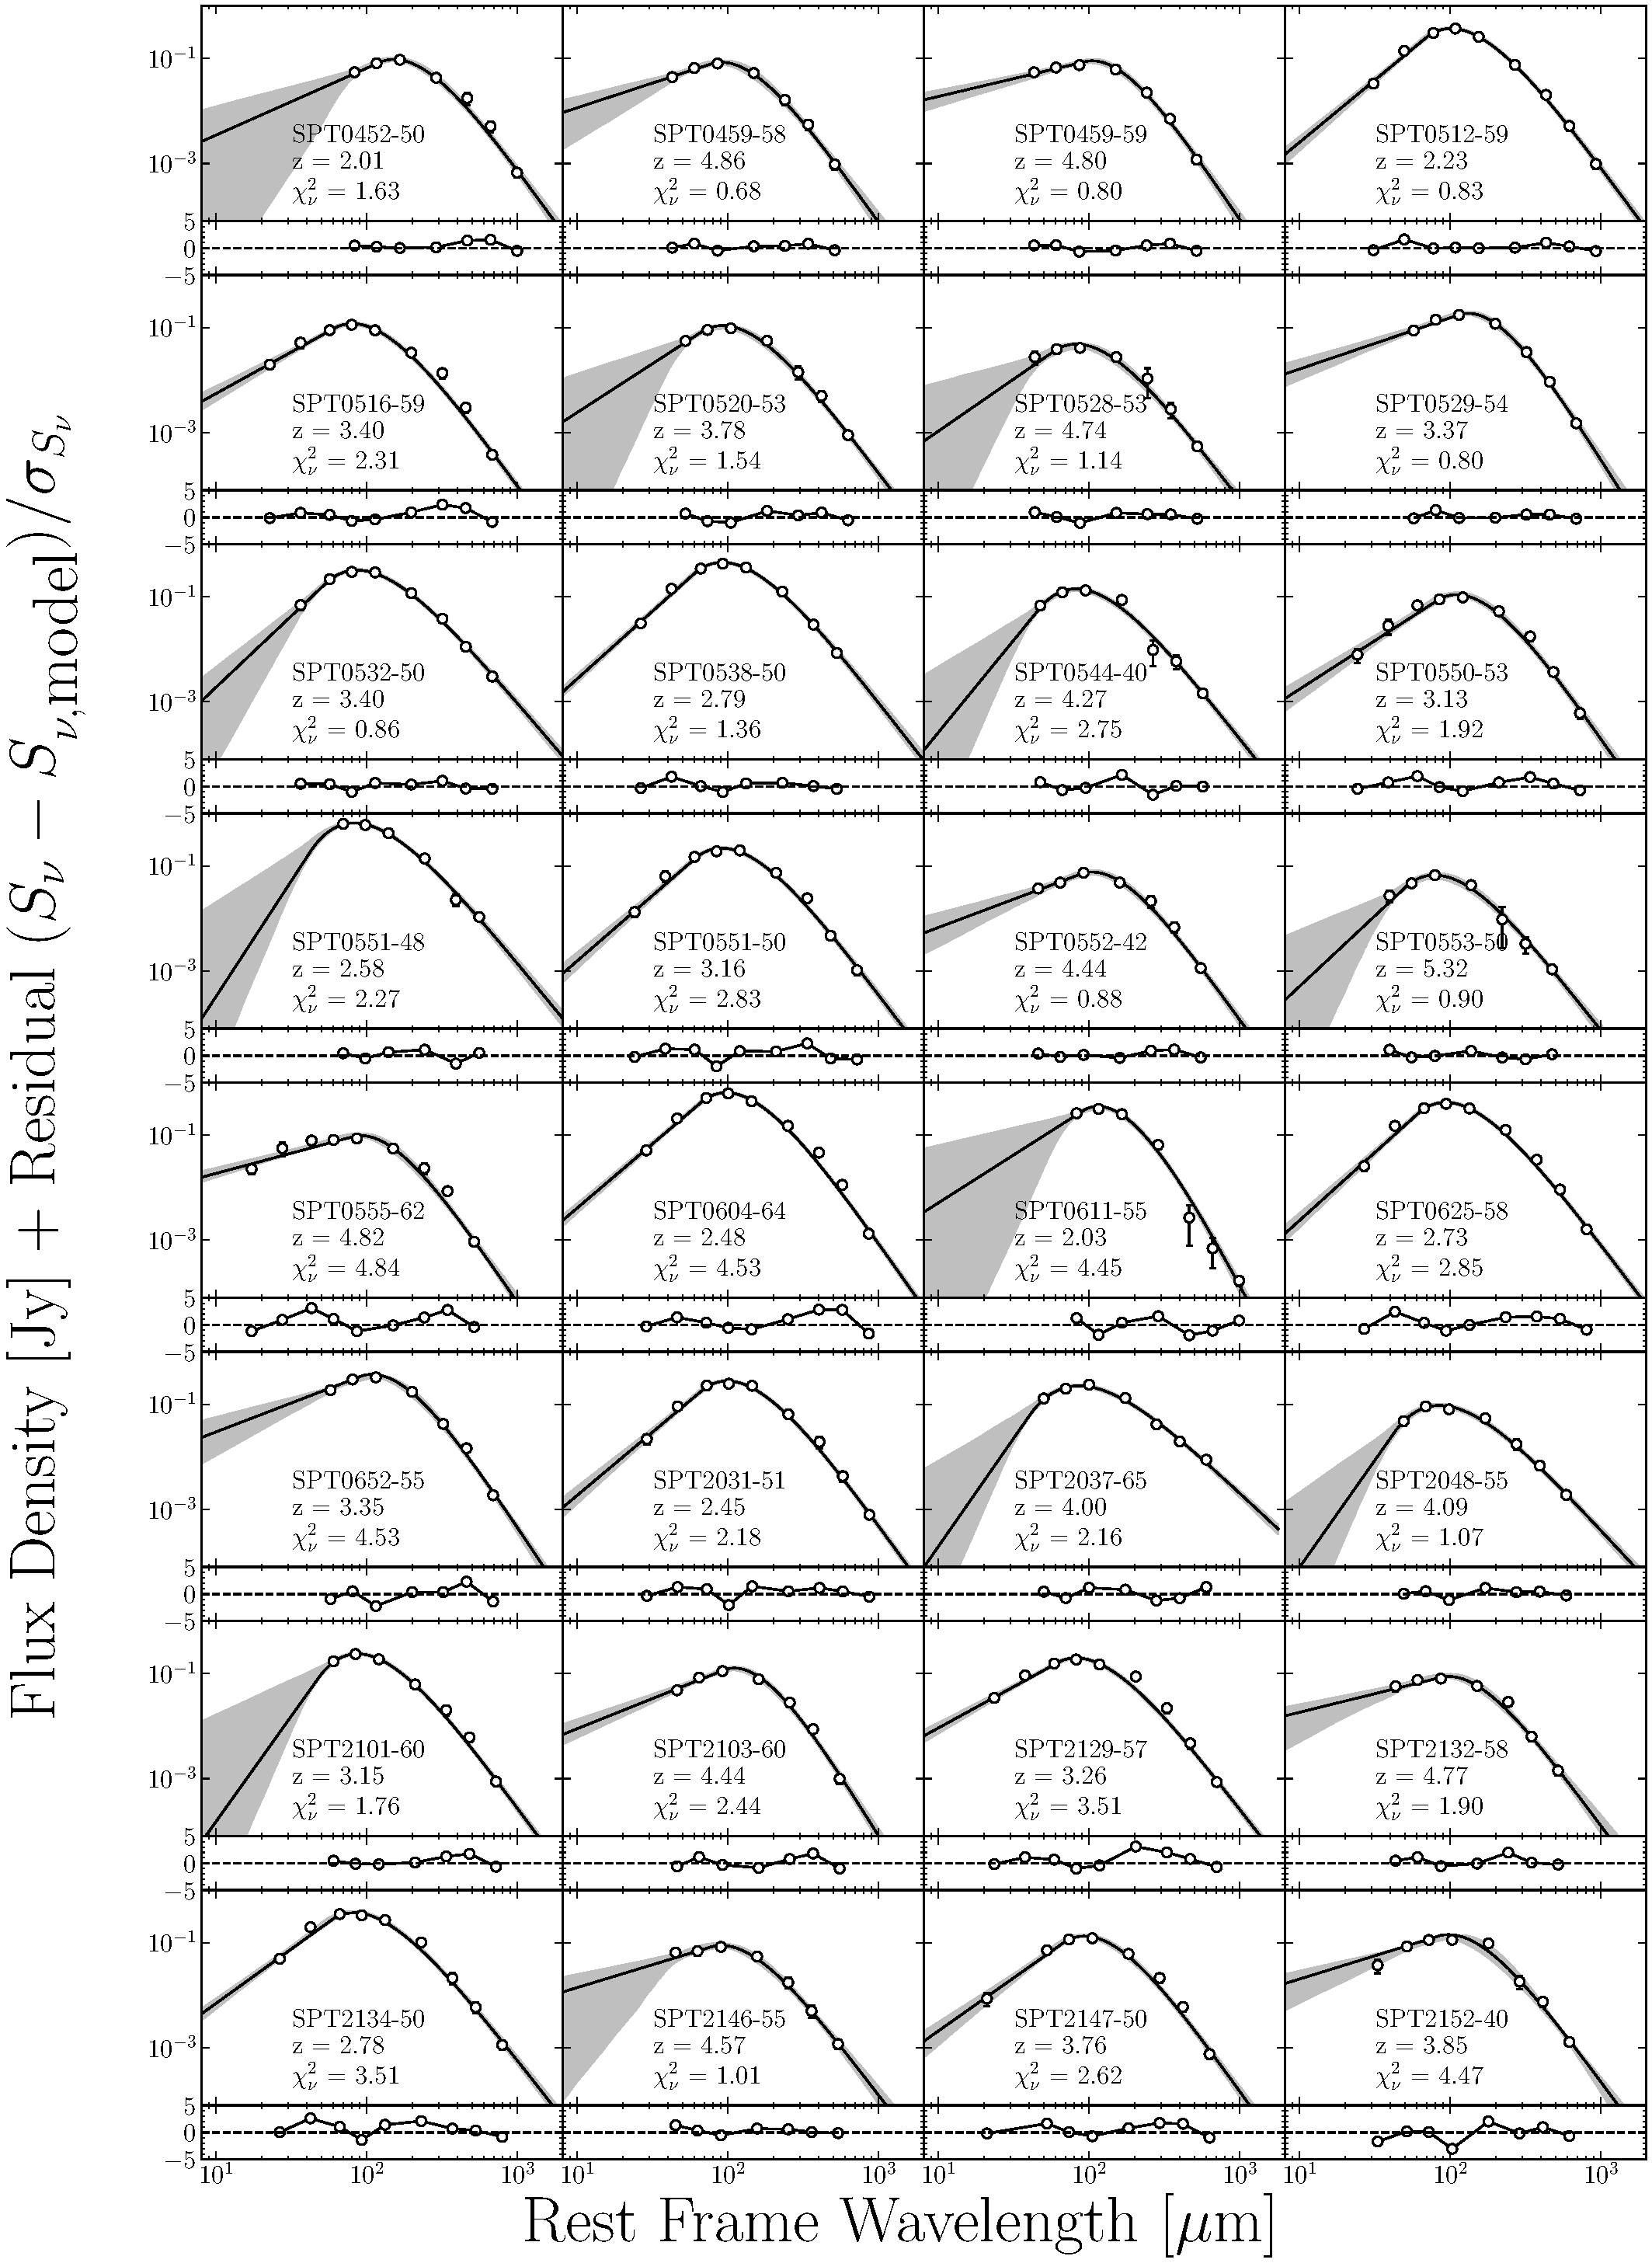
\includegraphics[width=\columnwidth]{Figures/Figure_D_1_part2.pdf}
\end{figure}
\begin{figure}
	\centering
	\includegraphics[width=\columnwidth]{Figures/Figure_D_1_part3.pdf}
\end{figure}


\begin{figure}
	\centering
	\caption[SEDs of SPT sample ($\lambda_1 = 100\,\mu$m)]{SEDs of the SPT sample ($\lambda_1 = 100\,\mu$m) and the residuals on the best fitting model. The shaded regions represent the $16$th to $84$th percentiles in the range of SEDs explored during fitting}
	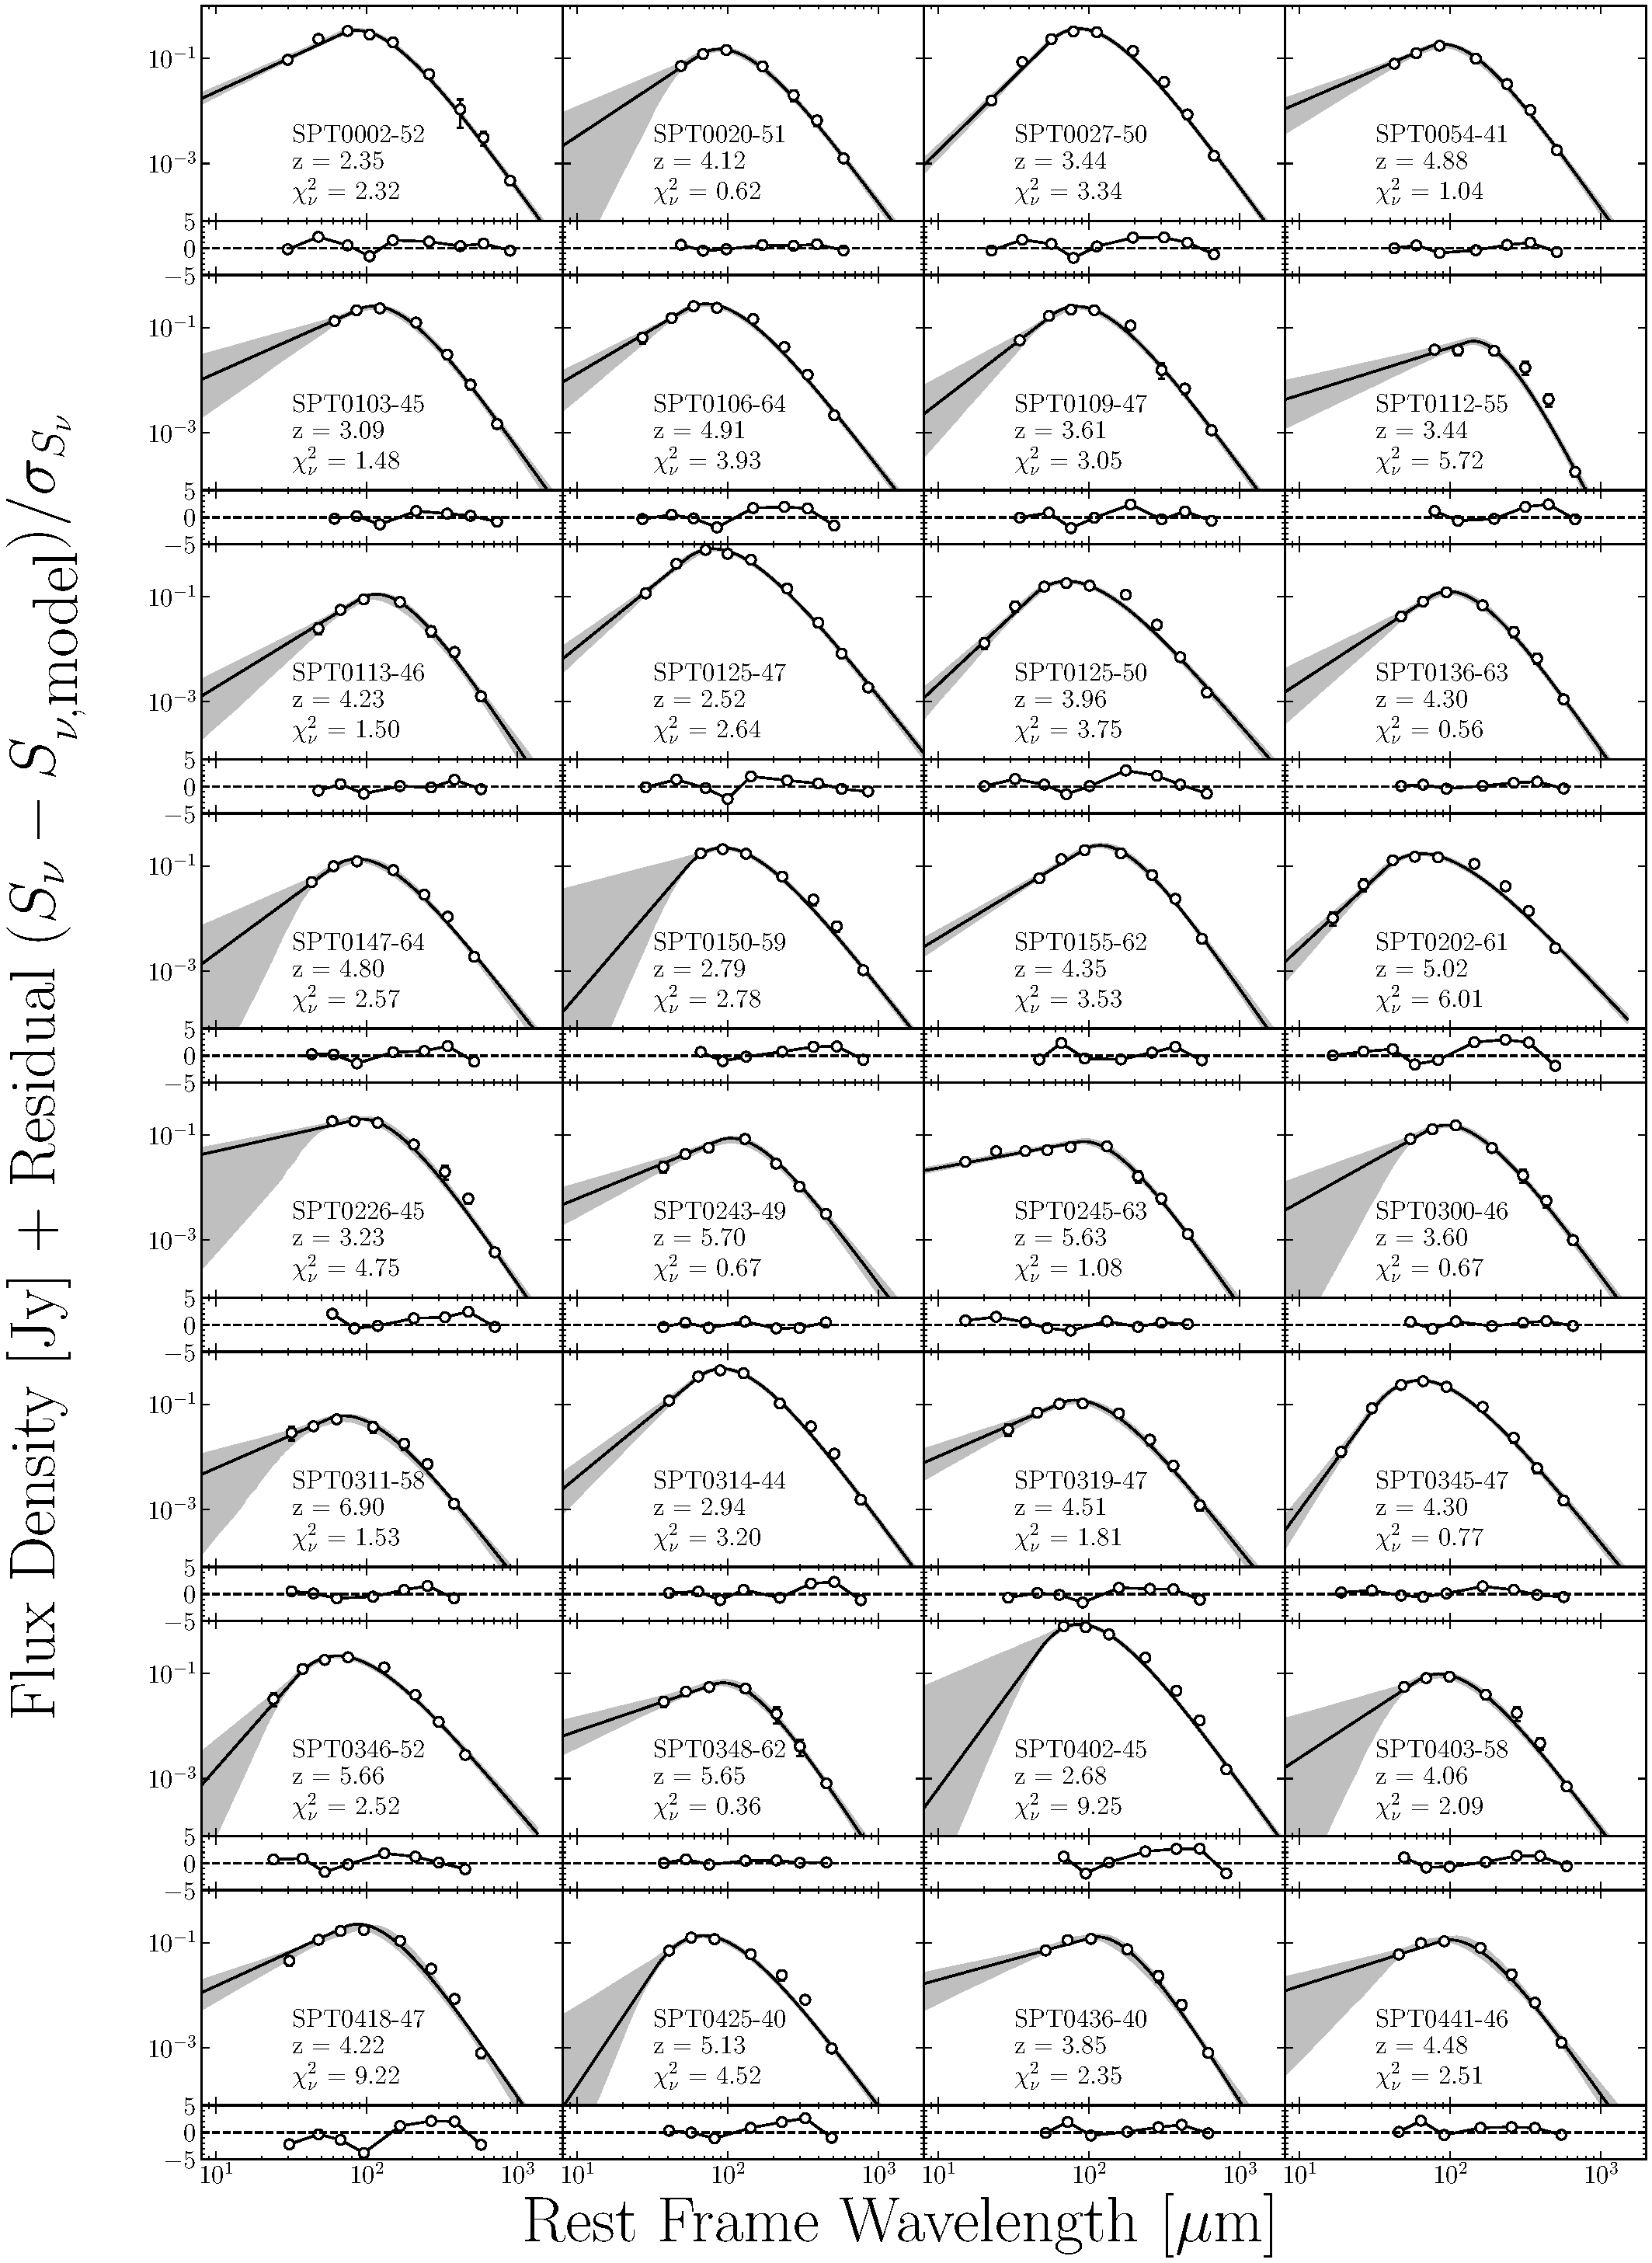
\includegraphics[width=\columnwidth]{Figures/Figure_D_2_part1.pdf}
\end{figure}
\begin{figure}
	\centering
	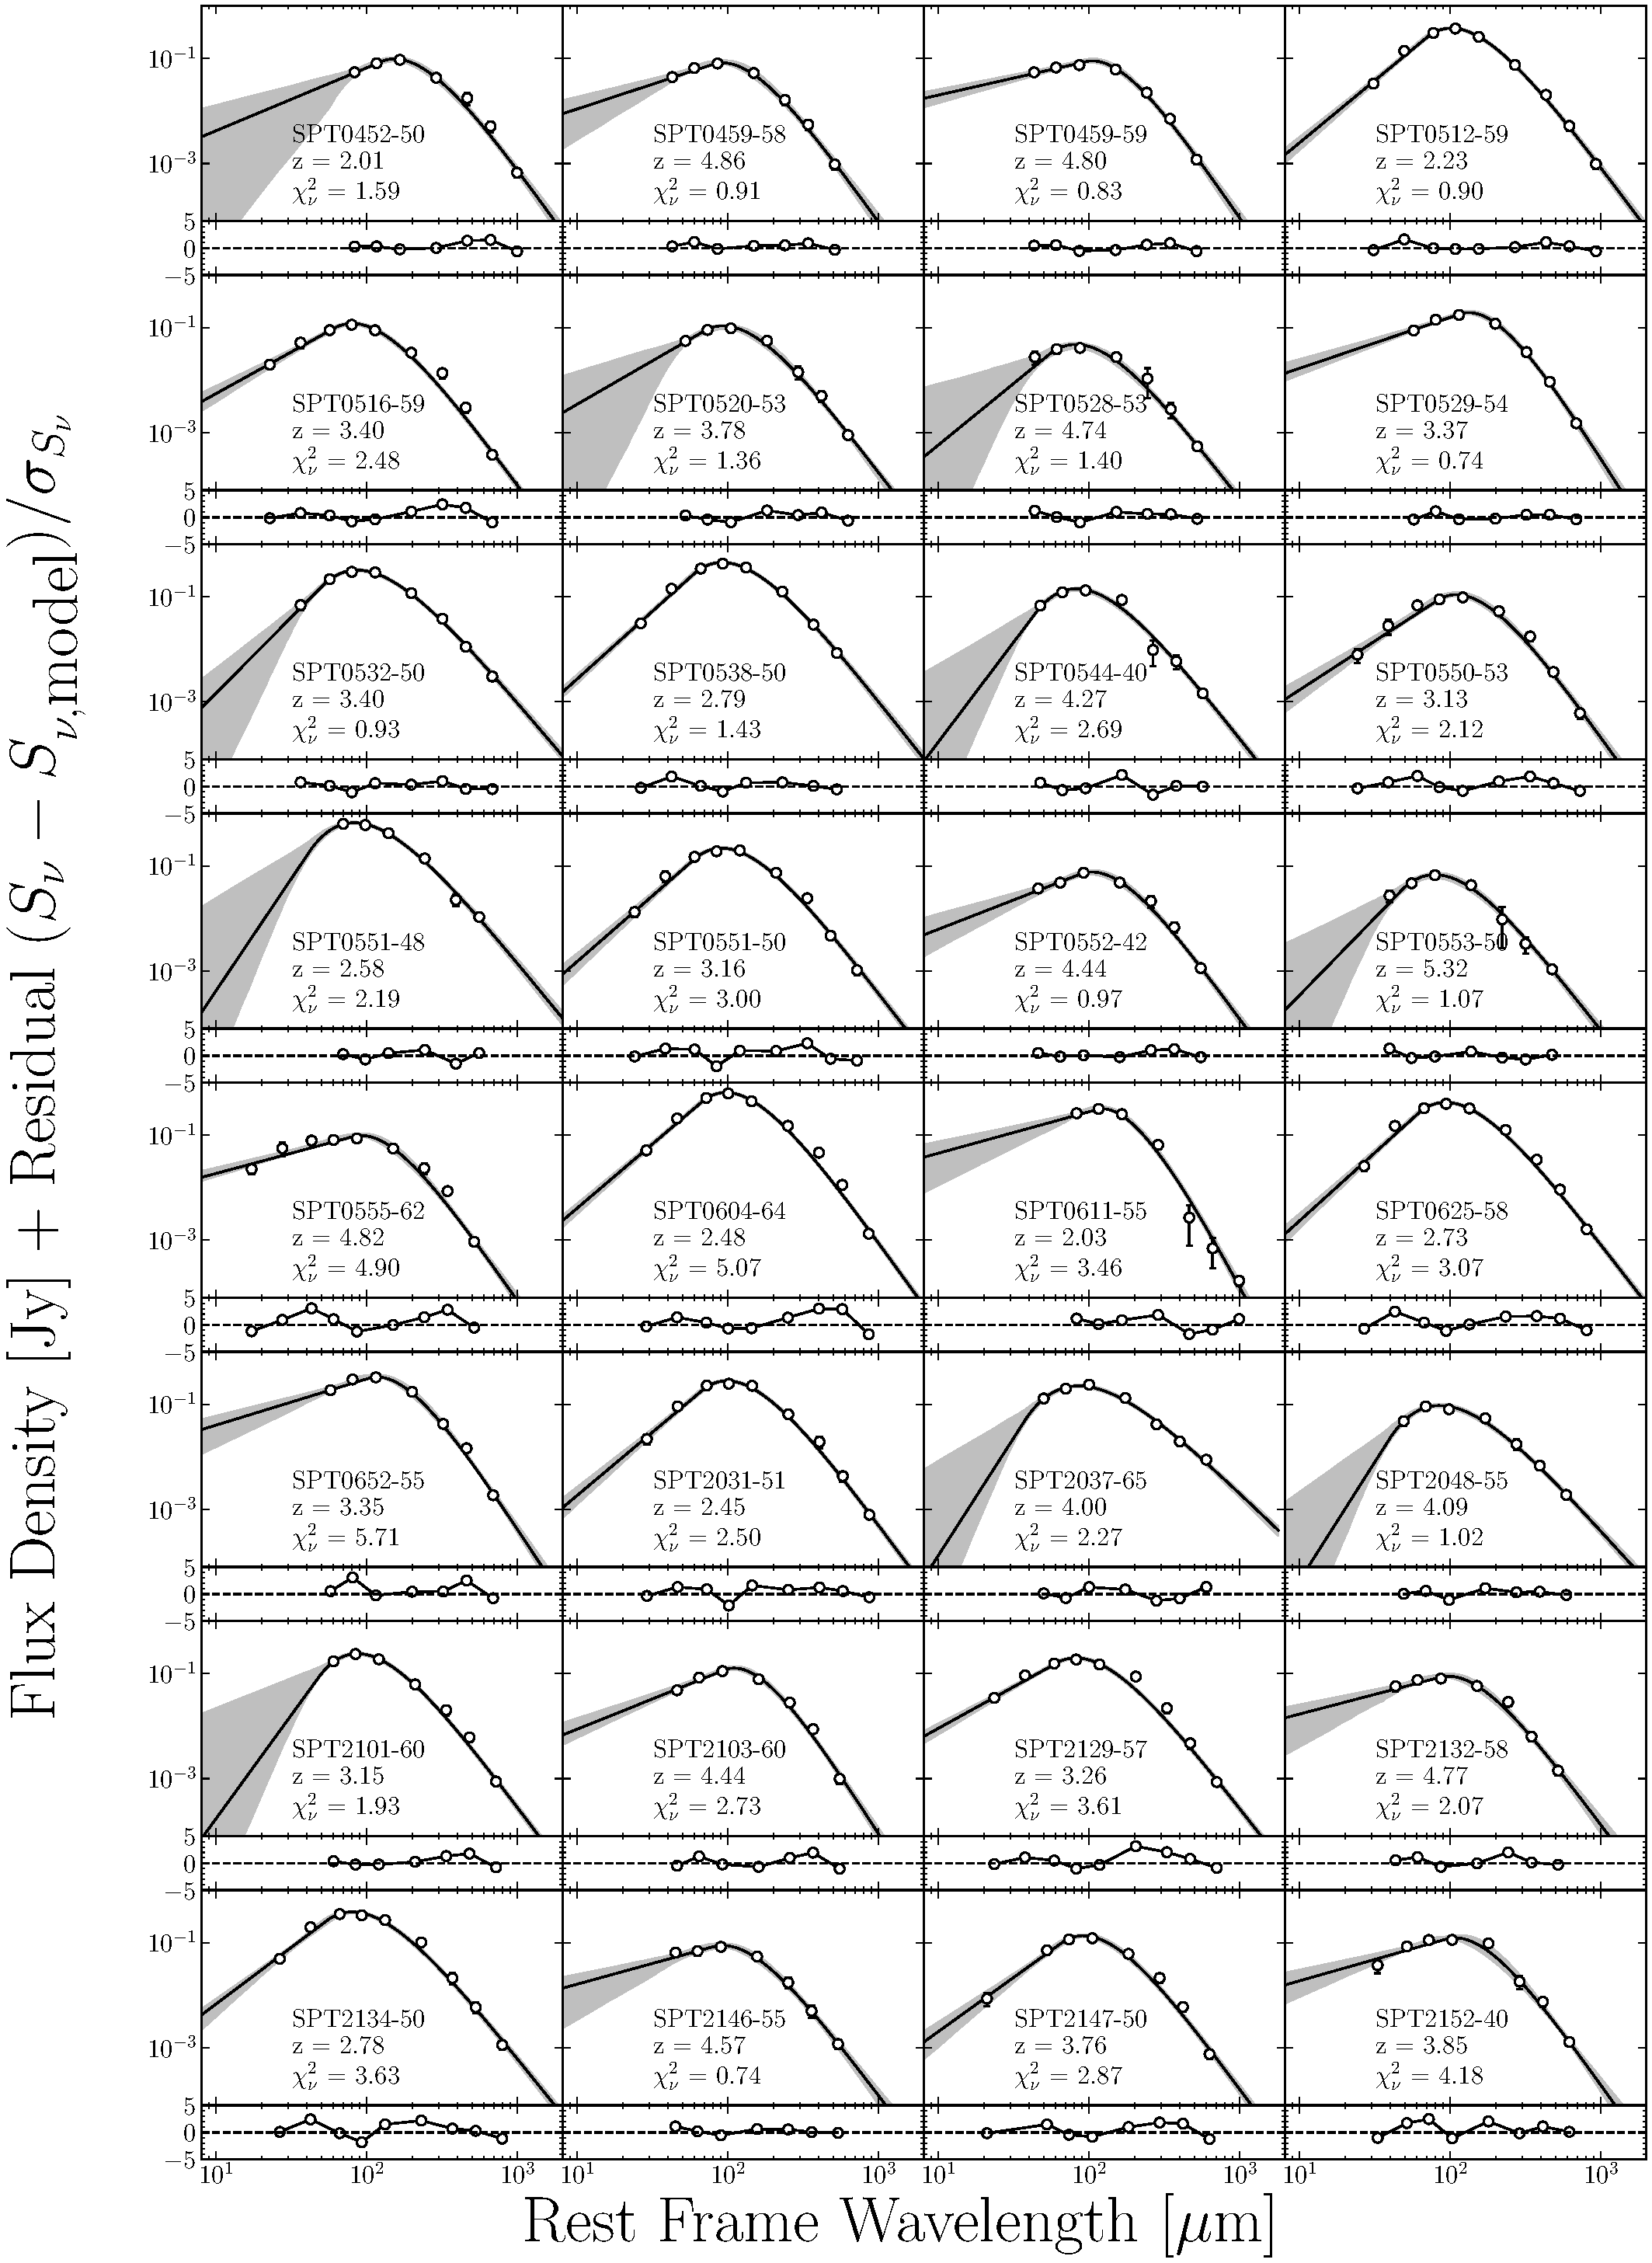
\includegraphics[width=\columnwidth]{Figures/Figure_D_2_part2.pdf}
\end{figure}
\begin{figure}
	\centering
	\includegraphics[width=\columnwidth]{Figures/Figure_D_2_part3.pdf}
\end{figure}


\begin{figure}
	\centering
	\caption[SEDs of SPT sample ($\lambda_1 = 200\,\mu$m)]{SEDs of the SPT sample ($\lambda_1 = 200\,\mu$m) and the residuals on the best fitting model. The shaded regions represent the $16$th to $84$th percentiles in the range of SEDs explored during fitting.}
	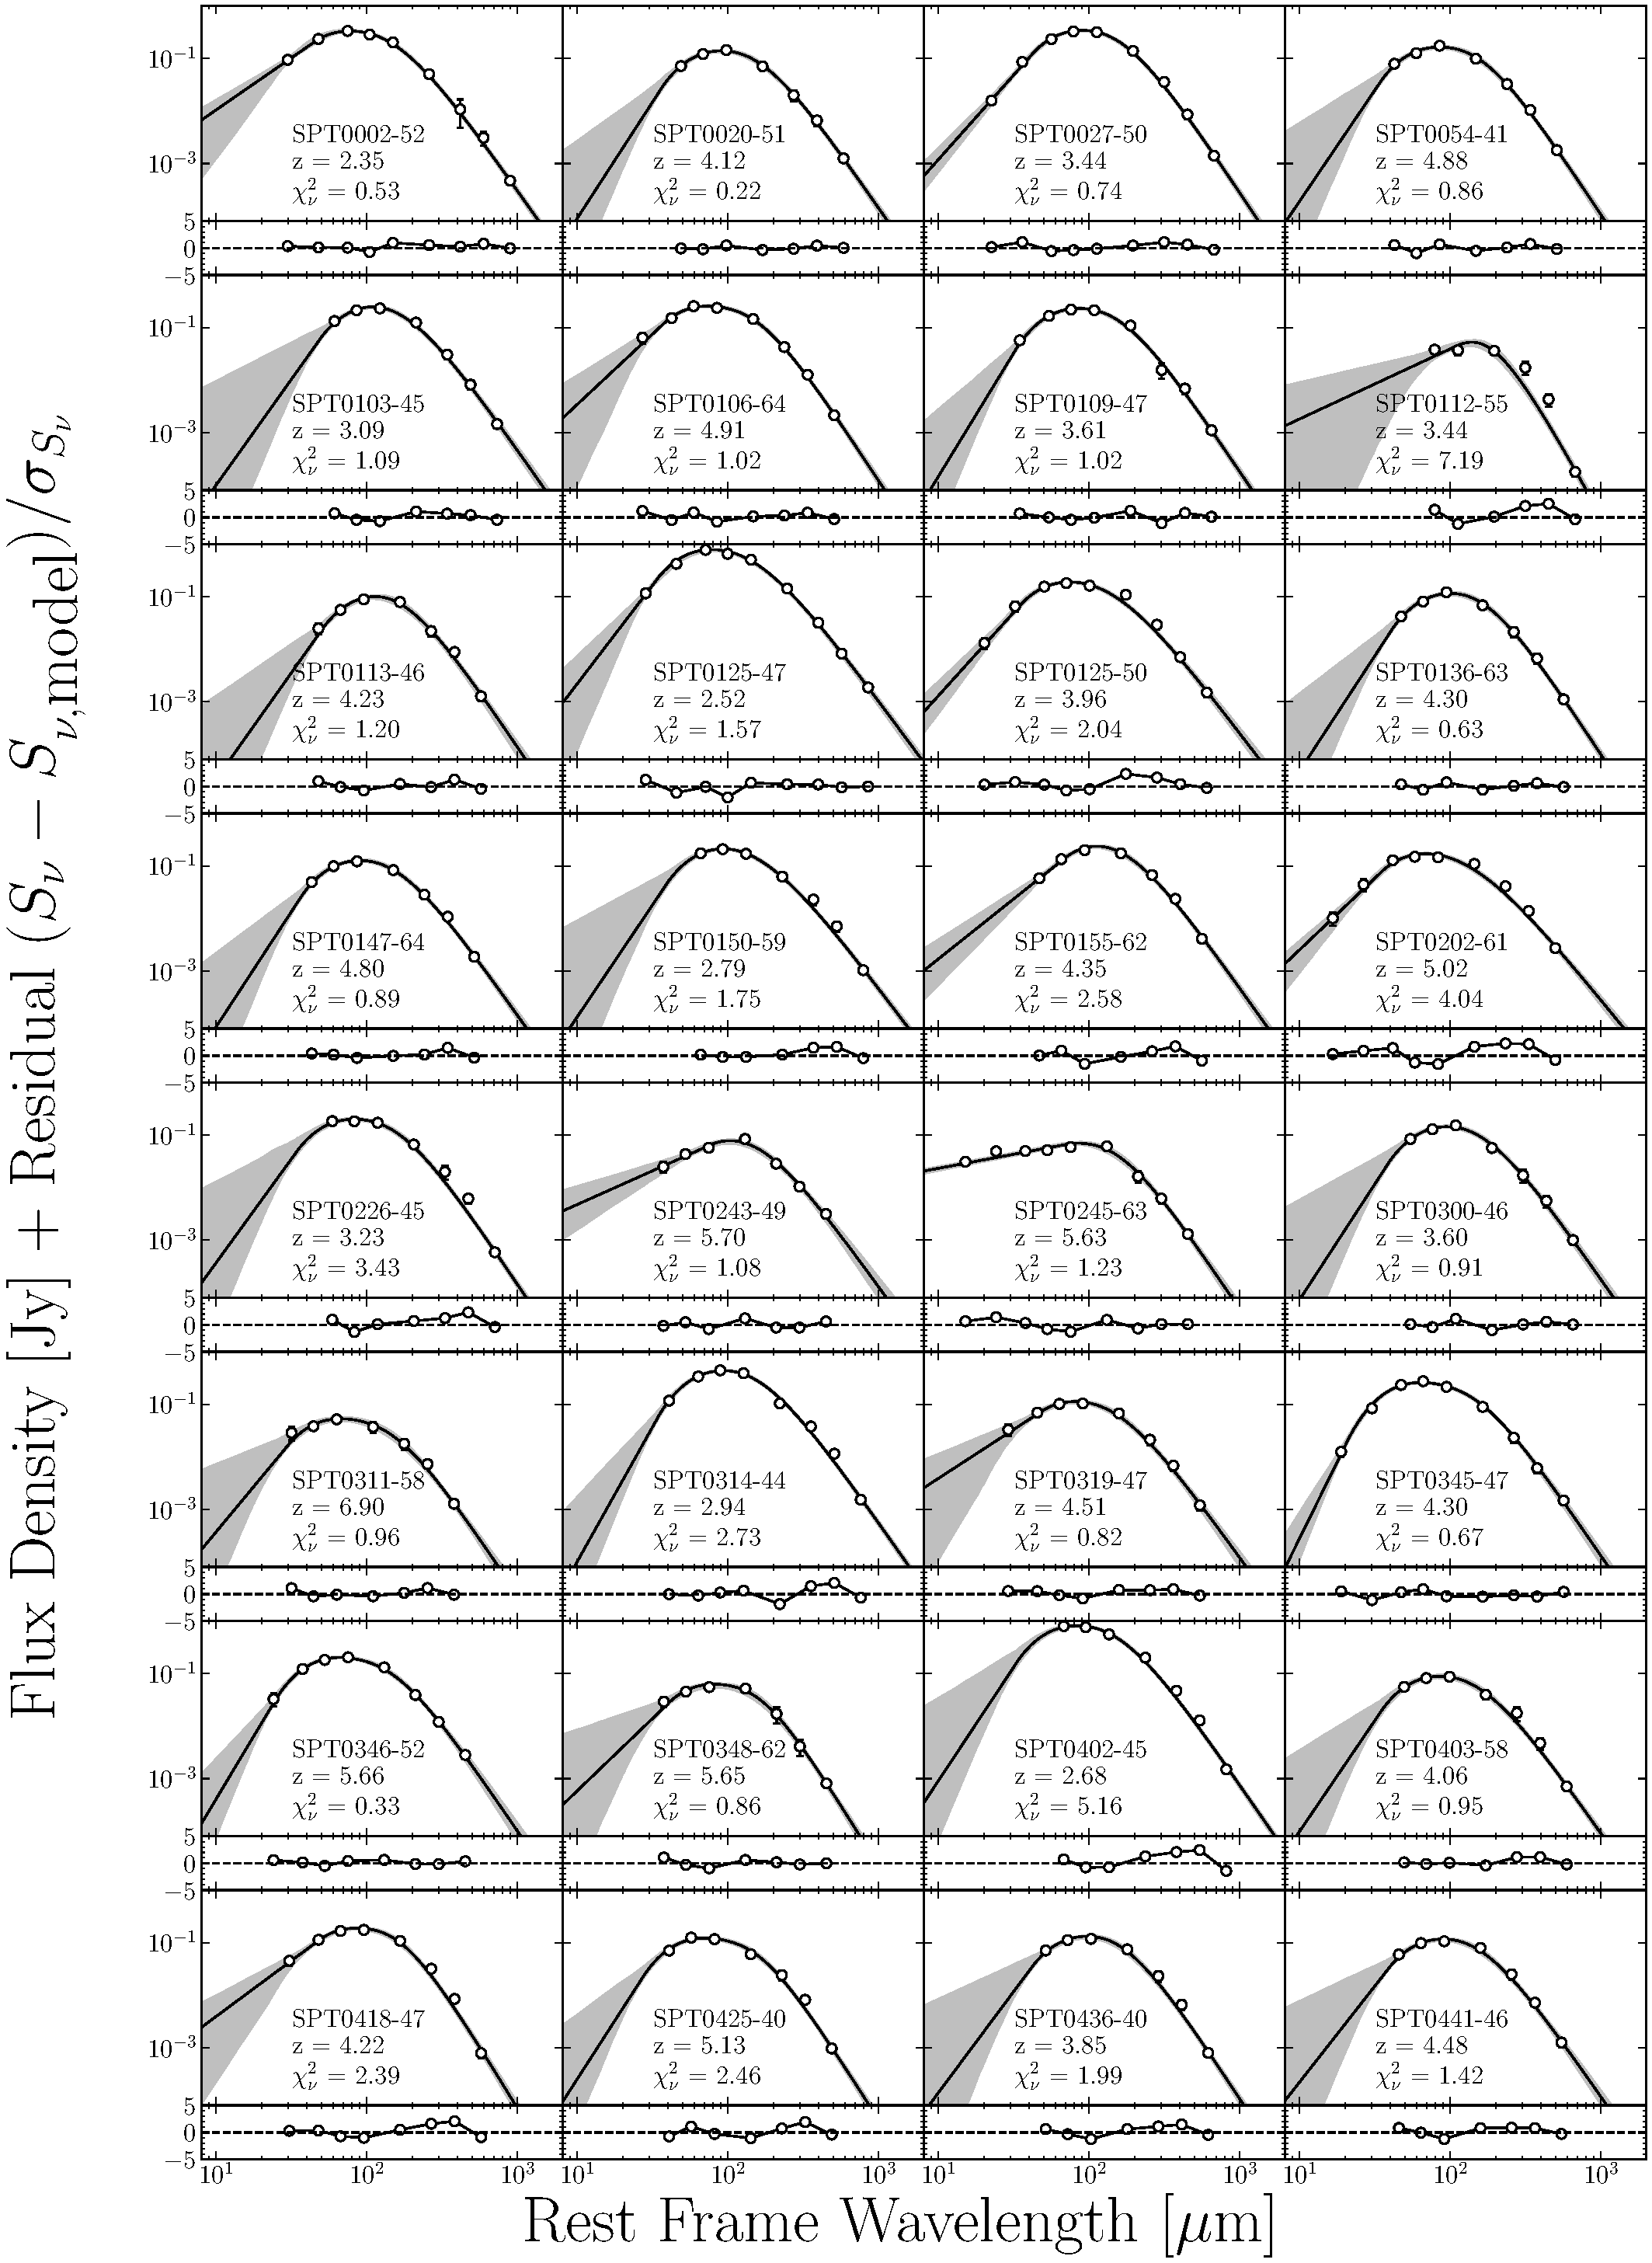
\includegraphics[width=\columnwidth]{Figures/Figure_D_3_part1.pdf}
\end{figure}
\begin{figure}
	\centering
	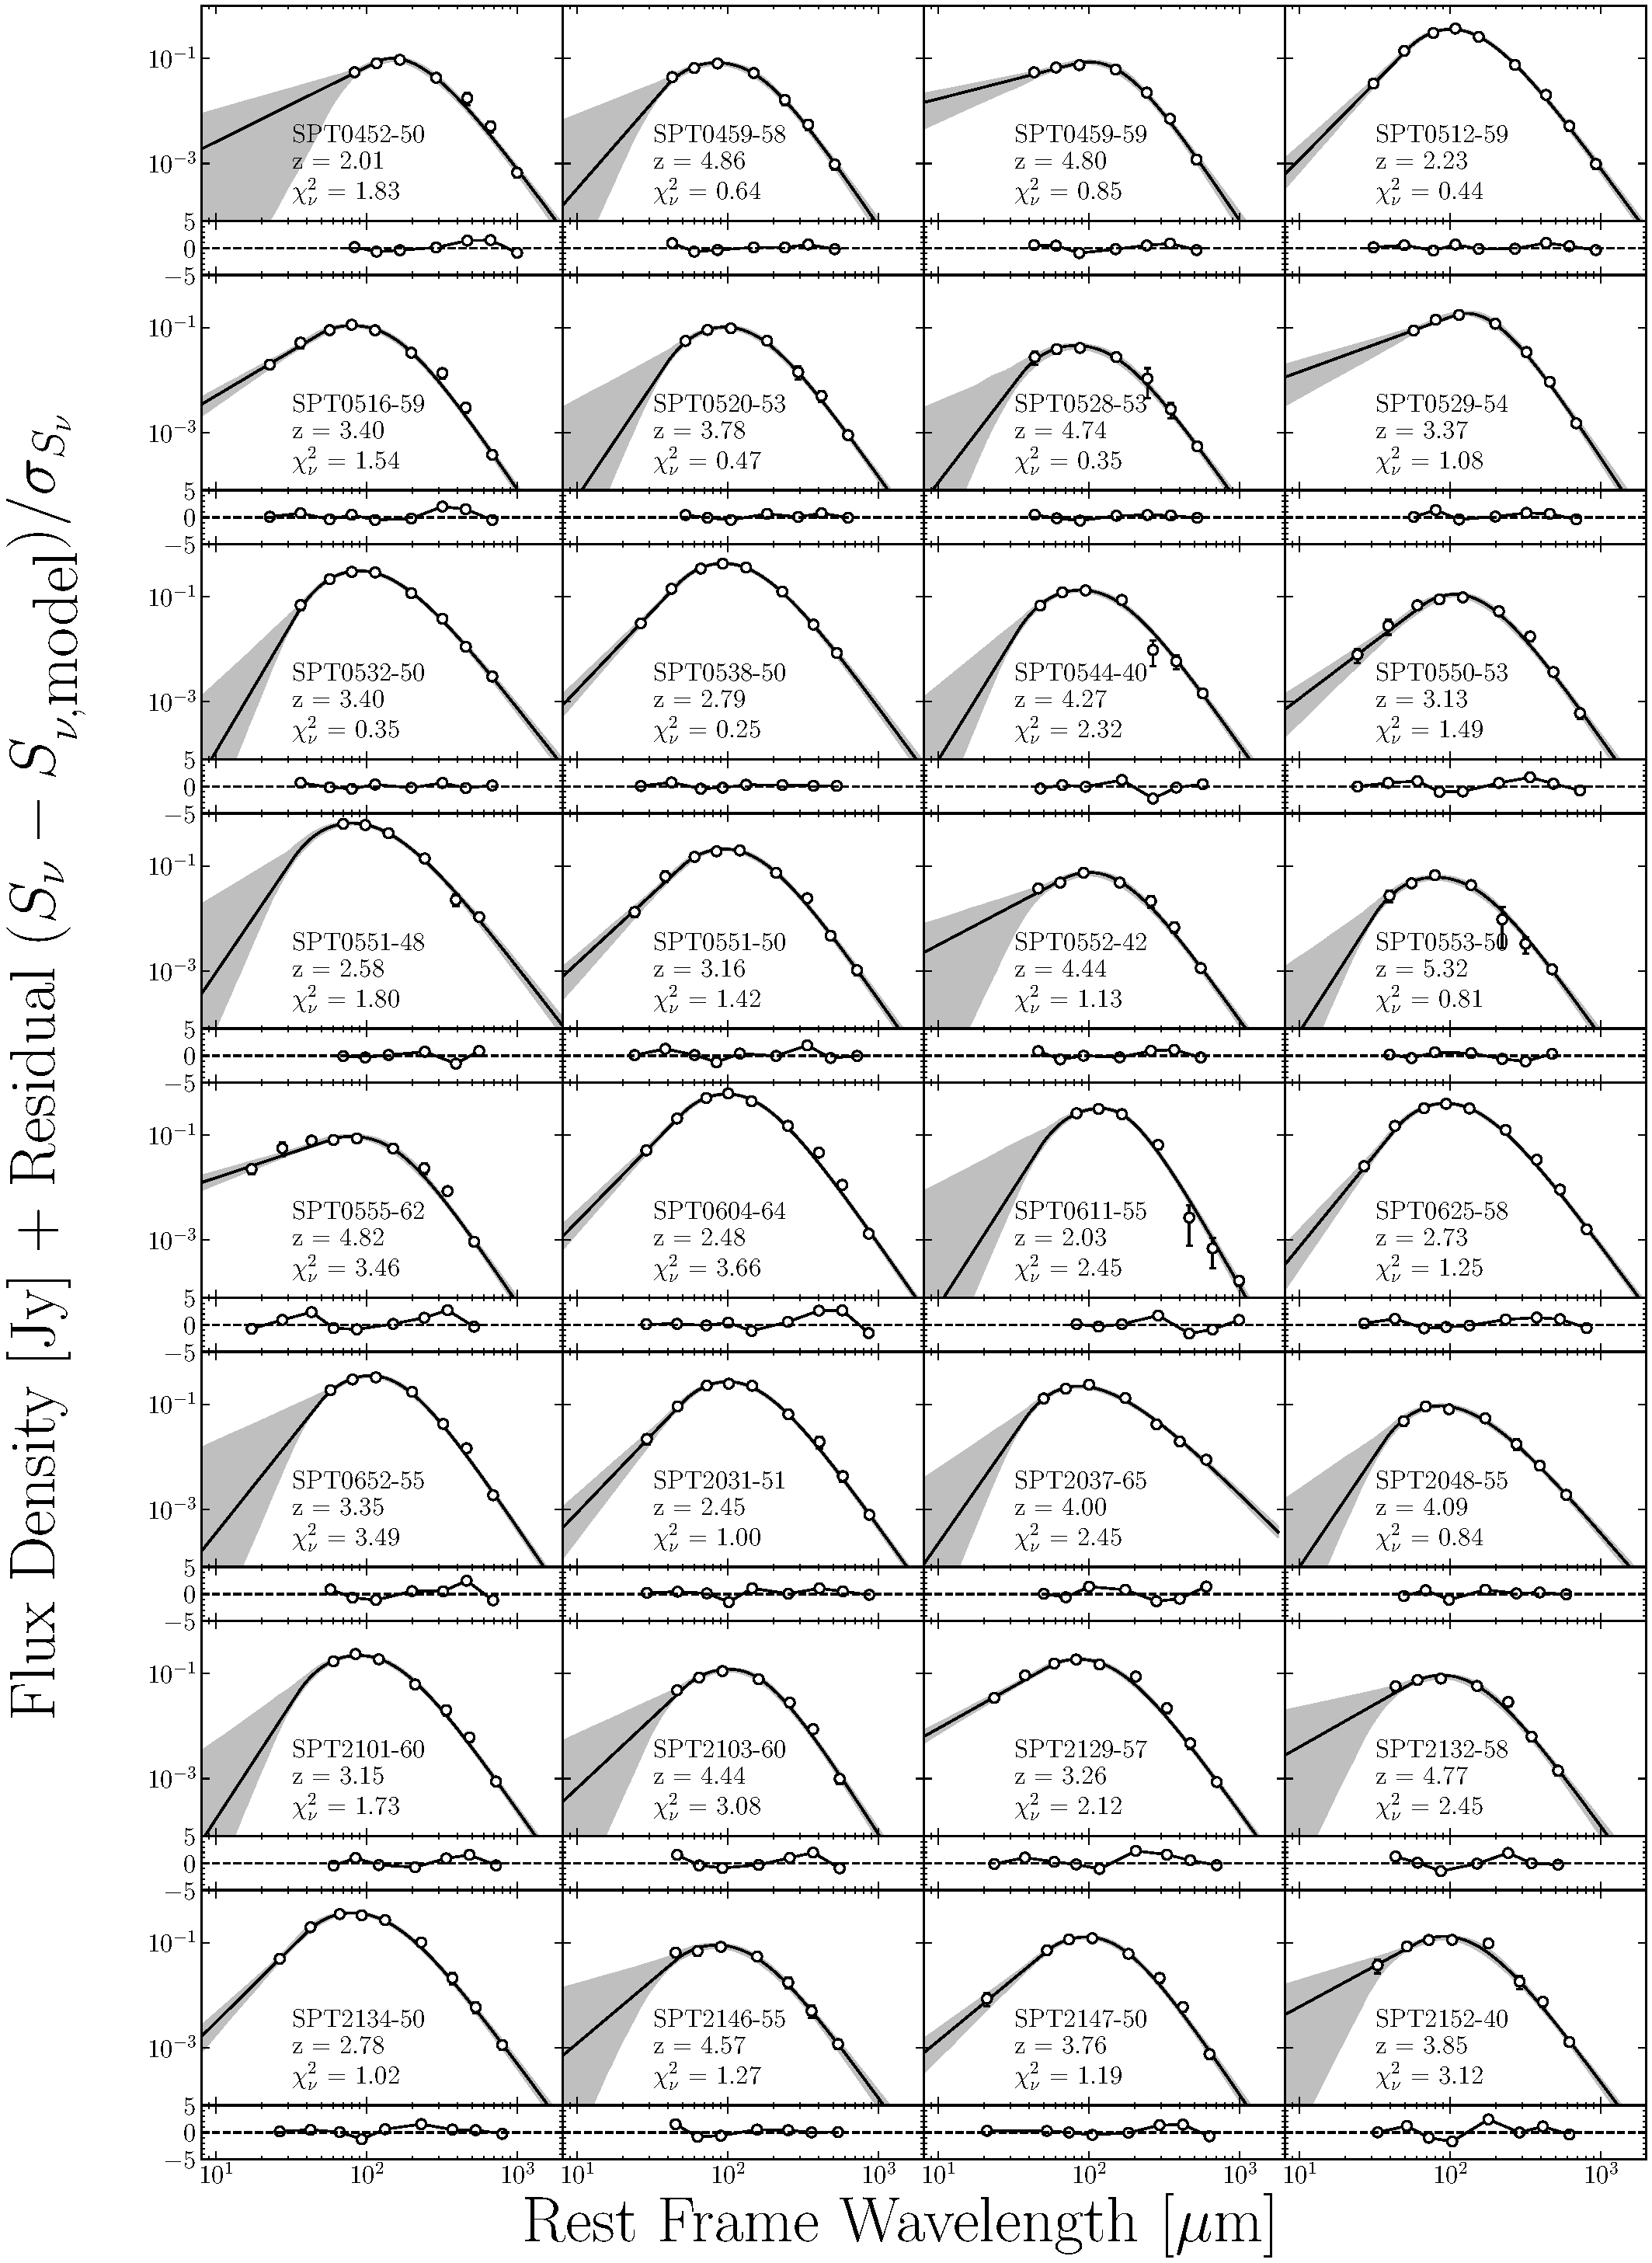
\includegraphics[width=\columnwidth]{Figures/Figure_D_3_part2.pdf}
\end{figure}
\begin{figure}
	\centering
	\includegraphics[width=\columnwidth]{Figures/Figure_D_3_part3.pdf}
\end{figure}
